\localauthor{Johann Schicho}

Im Entity-Relationship-Diagramm in Abbildung \ref{er:diagramm} sieht man die gesamte persistente Datenstruktur von LasEs. Die Kardinalität der \emph{Relationships} gibt die ganzzahligen Abhängigkeiten zwischen der einzelnen \emph{Entities} an. Die \emph{is-A} Spezialisierungen modellieren die unterschiedlichen Subtypen einer Entität. Ein im Diagramm doppelt umrandetes Entity ist ein \emph{schwaches} Entity. Das heißt, es existiert nur im Zusammenhang mit dem übergeordneten Entity. In unserem Fall kann beispielsweise kein Paper in der Datenbank existieren, ohne einer Einreichung zugeteilt zu sein.

\begin{figure}
	\centering
	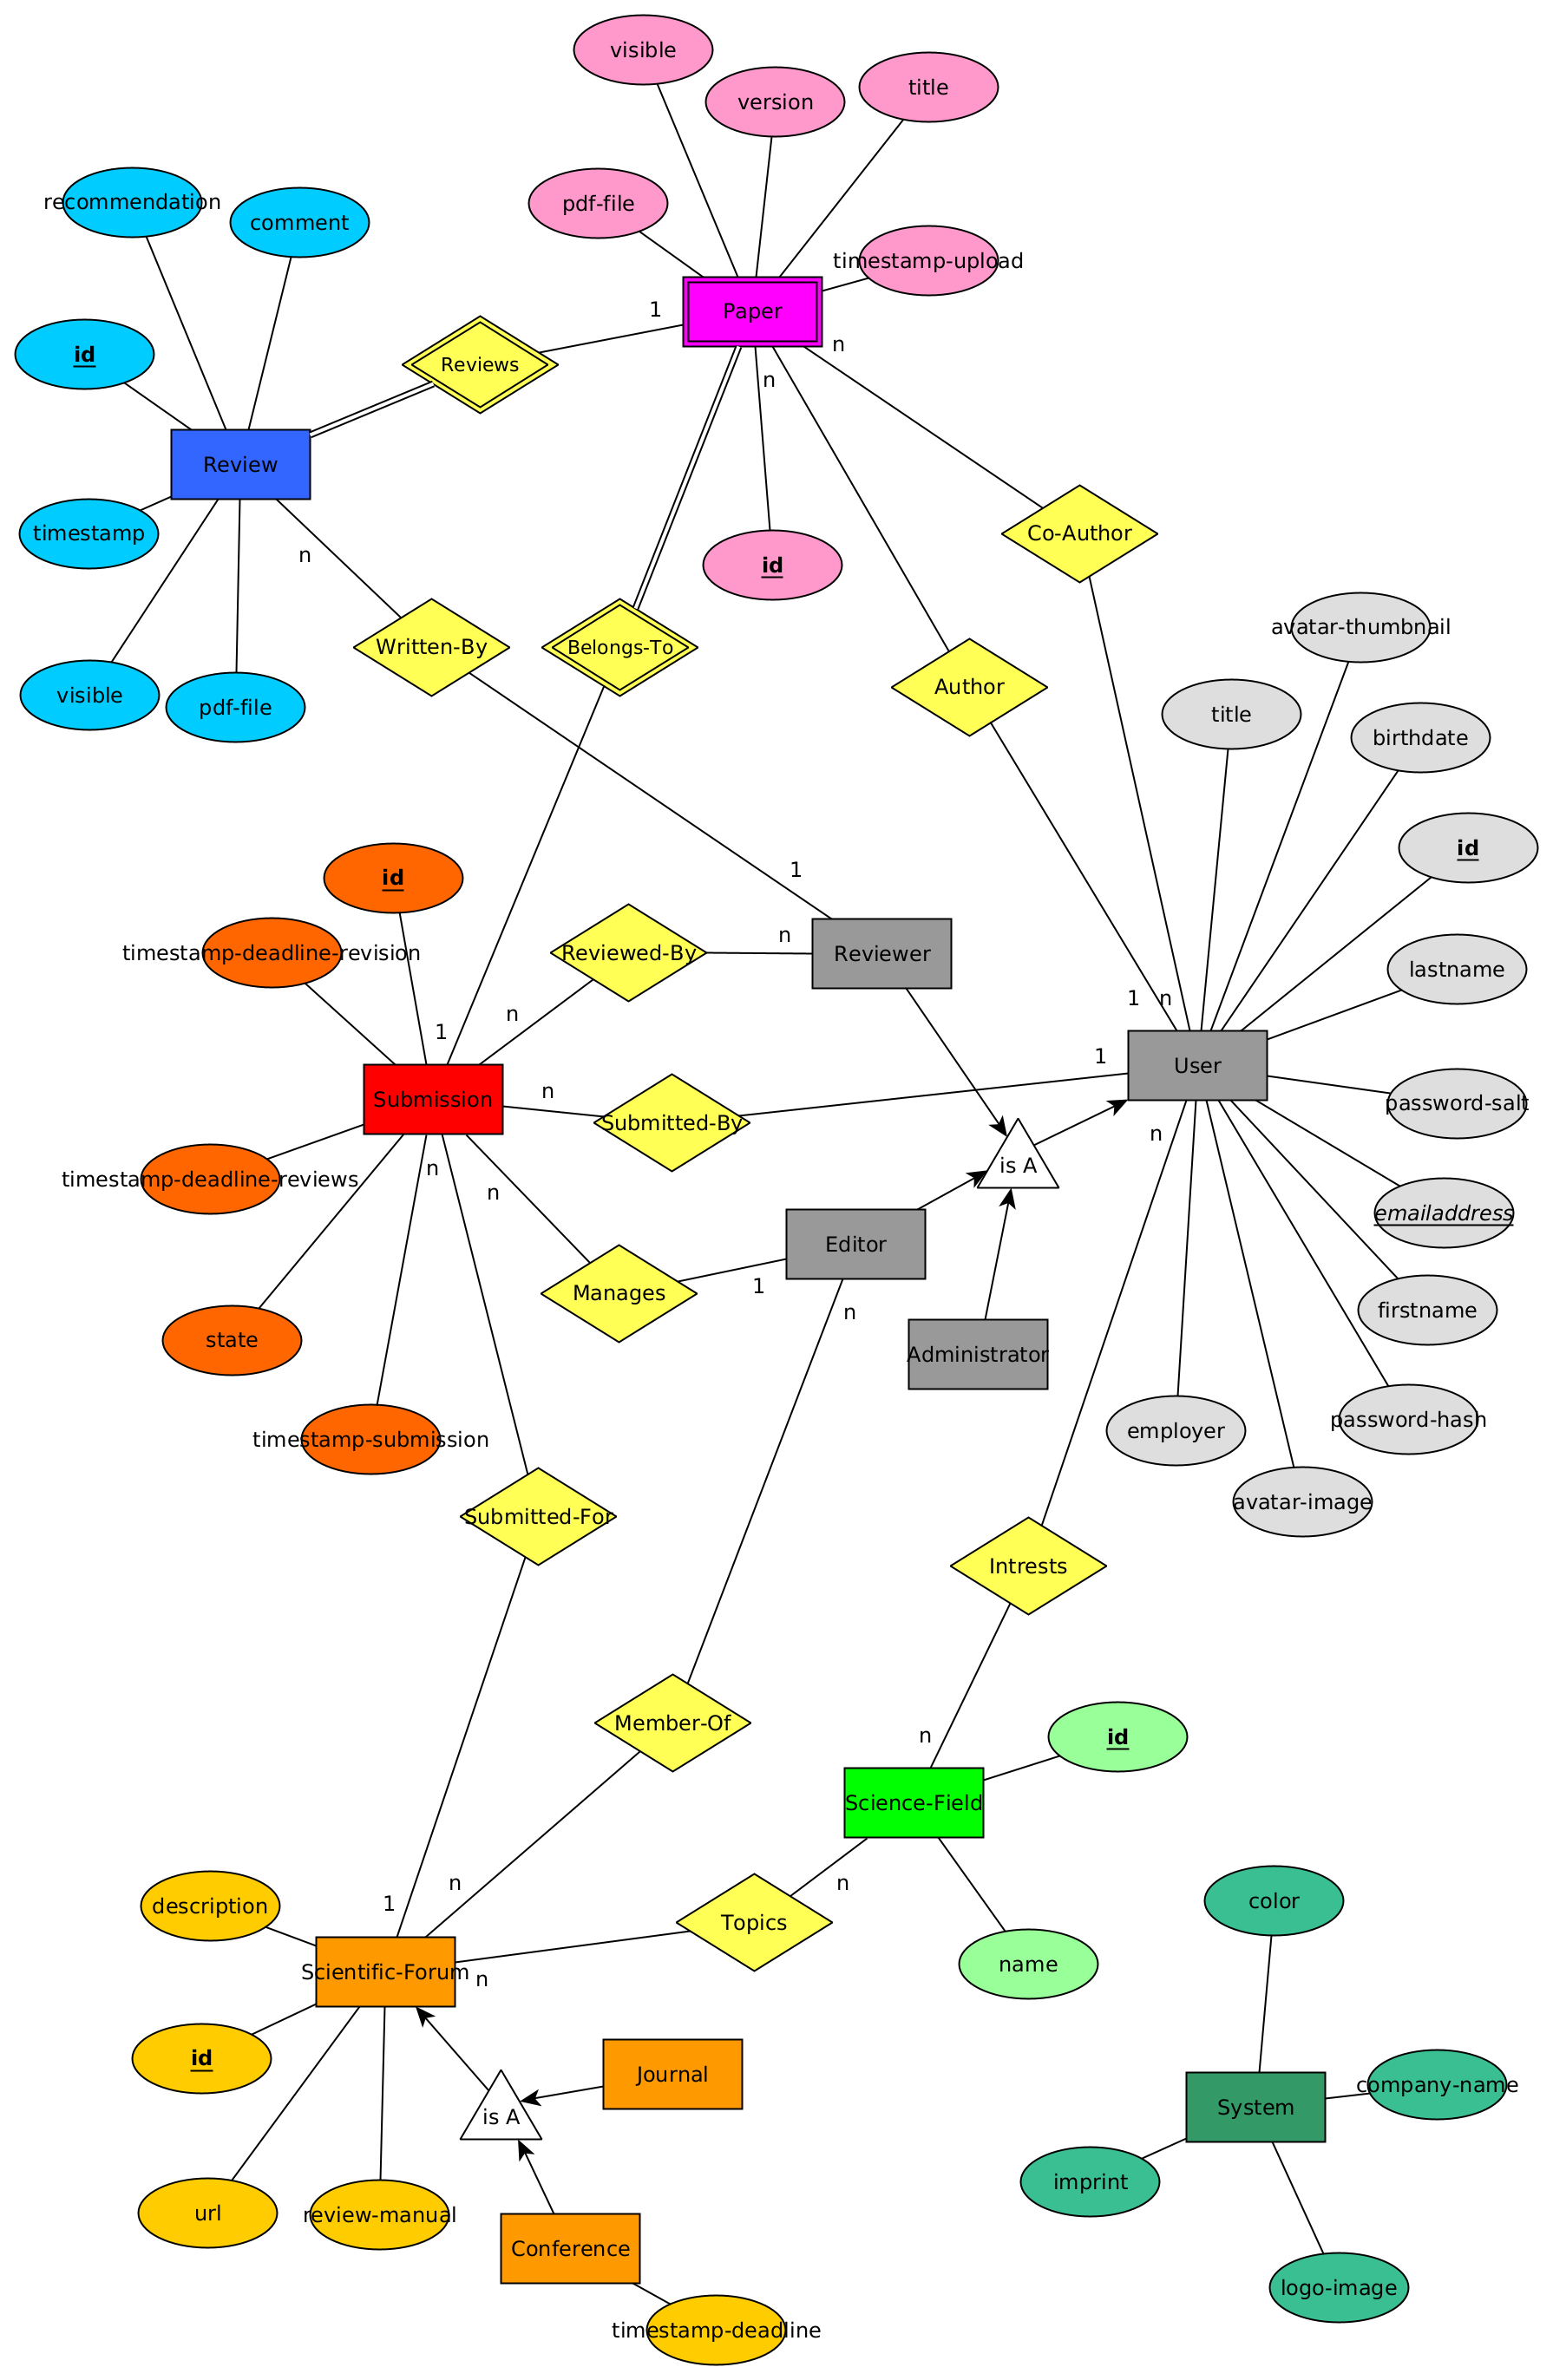
\includegraphics[width=\linewidth]{graphics/ER-Modell}
	\caption{Übersicht über die Zusammenhänge zwischen den Entitys}
	\label{er:diagramm}
\end{figure}

\subsection{Entities}

In Abbildung \ref{er:diagramm} werden die einzelnen Entities nochmal im Detail beschrieben. Mit der Notation \texttt{/DXXX/} wird sich auf die im Pflichtenheft aufgeführten Produktdaten bezogen.

\begin{description}
	\XXitem{User}{er:user} Ein Nutzer kann verschiedene Rollen wahrnehmen, diese werden durch die \emph{is-A}-Spezifizierung modelliert. Die Attribute entsprechen den in \texttt{\textbf{/D010/}} und \texttt{\textbf{/DW015/}} angegebenen Daten.

	\XXitem{Verification}{er:verification} Da jede E-Mailadressenänderung eine Verifizierung benötigt, werden hier die Daten, zu welchen geändert wird, gespeichert. Das \emph{validation-random} ist dabei der String, welcher im Verifizierungslink per E-Mail versendet wird.

	\XXitem{Paper}{er:paper} Ein Paper ist das in einem Einreichungsprozess hochgeladene Paper. Es ist modelliert als eine schwache Entität, abhängig von einer Einreichung, da ein Paper nicht im System existieren kann, ohne zu einem Einreichungsprozess zugeordnet zu werden. Es speichert die in \texttt{\textbf{/D020/}} angegebenen Daten.

	\XXitem{Submission}{er:submission} Eine Einreichung speichert alle zu einem Einreichungsprozess gehörenden Daten, inklusive der Metadaten, wie den Einreicher und Ko-Autor, also alle in \texttt{\textbf{/D025/}} und \texttt{\textbf{/DW021/}} angegebenen Daten.

	\XXitem{Review}{er:review} Ein Gutachten ist immer genau einem Paper zugeordnet, welches wiederum genau einer Einreichung zugeordnet ist. Es speichert die PDF als binäres Attribut in der Datenbank ab und alle zugehörigen Metadaten.
	Damit spiegelt es \texttt{\textbf{/D040/}} wieder.

	\XXitem{Scientific Forum}{er:forum} Ein wissenschaftliches Forum besitzt die Referenz auf alle zu diesem Journal/Konferenz eingereichten Papers. Zusätzlich sind allgemeine Metadaten abgespeichert. Damit erfüllt es \texttt{\textbf{/D030/}}

	\XXitem{Scientific Field}{er:field} Liste aller Fachgebiete bzw. Interessengebiete, die in LasEs verwendet werden. Diese werden als Fachgebieten der Foren und als Forschungsinteressen der Nutzer verwendet. Nach \texttt{\textbf{/D035/}}.

	\XXitem{System}{er:system} Systemdaten speichern allgemeine Informationen über die Firma, die LasEs einsetzt. Sie sind in \texttt{\textbf{/D050/}} spezifiziert.

\end{description}
